\documentclass[fleqn,12pt]{article}
\usepackage{mycommands,amssymb,amsmath,amsthm,color,pagesize,outlines,cite,subfigure}
\usepackage[small]{caption}
\usepackage[pdftex]{epsfig}
%\usepackage{mathtools}

\usepackage[round]{natbib}

% for algorithm
\usepackage[noend]{algpseudocode}
\usepackage{algorithm}

%\addtolength{\evensidemargin}{-.5in}
%\addtolength{\oddsidemargin}{-.5in}
%\addtolength{\textwidth}{0.9in}
%\addtolength{\textheight}{0.9in}
%\addtolength{\topmargin}{-.4in}

% measurements for 1 inch margin
\addtolength{\oddsidemargin}{-.875in}
\addtolength{\evensidemargin}{-.875in}
\addtolength{\textwidth}{1.75in}
\addtolength{\topmargin}{-.875in}
\addtolength{\textheight}{1.75in}

\usepackage{hyperref} % for linking references 
\usepackage{setspace}
\usepackage{stackrel}
\usepackage{flafter} % section title after figure
\doublespacing

%% Appendix theorem counter
\usepackage{chngcntr}
\usepackage{apptools}
\AtAppendix{\counterwithin{Theorem}{section}}

%\DeclareMathOperator*{\vec}{vec}
\DeclareMathOperator*{\diag}{diag}
\DeclareMathOperator*{\Tr}{Tr}
\DeclareMathOperator*{\argmin}{arg\,min}
\DeclareMathOperator*{\argmax}{arg\,max}
\DeclareMathOperator*{\ve}{\text{vec}}
\DeclareMathOperator*{\Th}{\text{th}}

% If your paper is accepted, change the options for the package
% aistats2017 as follows:
%
%\usepackage[accepted]{aistats2017}
%
% This option will print headings for the title of your paper and
% headings for the authors names, plus a copyright note at the end of
% the first column of the first page.


\begin{document}

\newtheorem{Theorem}{Theorem}[section]
\newtheorem{Lemma}[Theorem]{Lemma}
\newtheorem{Corollary}[Theorem]{Corollary}
\newtheorem{Proposition}[Theorem]{Proposition}
\newtheorem{Conjecture}[Theorem]{Conjecture}
\theoremstyle{definition} \newtheorem{Definition}[Theorem]{Definition}

\title{Nonconvex penalized regression using depth-based penalty functions: multitask learning and support union recovery in high dimensions}
\date{}
\author{Subhabrata Majumdar, Snigdhansu Chatterjee}
\maketitle


\begin{abstract}
We propose a new class of nonconvex penalty functions in the paradigm of multitask sparse penalized regression that are based on data depth-based inverse ranking. Focusing on a one-step sparse estimator of the coefficient matrix using local linear approximation of the penalty function, we derive its theoretical properties and provide the algorithm for its computation. For orthogonal design and independent responses, the resulting thresholding rule enjoys near-minimax optimal risk performance, similar to the adaptive lasso \citep{Zou06}. A simulation study as well as real data analysis demonstrate its effectiveness compared to present methods that provide sparse solutions in multivariate regression.
\end{abstract}


\vspace{.5cm}

\textbf{Keywords:} multivariate regression, nonconvex penalties, data depth, sparse regression, high-dimensional data

\newpage

\section{Introduction}

Consider the multitask linear regression model:
%
$$ \bfY = \bfX \bfB + \bfE $$
%
where $\bfY \in \mathbb R^{n\times q}$ is the matrix of responses, and $\bfE$ is $n\times q$ the noise matrix: each row of which is drawn from $\mathcal{N}_q ({\bf 0}_q, \bfSigma)$ for a $q \times q$ positive definite matrix $\bfSigma$. We are interested in sparse estimates of the coefficient matrix $\bfB$ through solving penalized regression problems of the form
%
\begin{equation}\label{eqn:penEqn}
\min_\bfB \Tr \{ (\bfY - \bfX\bfB)^T ( \bfY - \bfX\bfB) \} + P_\lambda(\bfB)
\end{equation}
%
The frequently studied classical linear model may be realized as a special case of this 
for $q = 1$, where given a size-$n$ sample of random responses $\bfy = (y_1, y_2, ..., y_n)^T$ and $p$-dimensional predictors $\bfX = (\bfx_1, \bfx_2, ...,\bfx_n)^T$, the 
above model may now be written as:
%
$$
\bfy = \bfX \bfbeta + \bfepsilon; \quad \bfepsilon = (\epsilon_1,...,\epsilon_n)^T \sim \mathcal N_n ({\bf 0}_n, \sigma^2\bfI_p).
$$
%

Here the typical objective is to estimate the parameter vector $\bfbeta$ by minimizing $\sum_{i=1}^n \rho ( y_i - \bfx_i^T \bfbeta)$, for some loss function $\rho(.)$. Selecting important variables in this setup is often significant from an inferential and predictive perspective it is generally achieved by obtaining an estimate of $\bfbeta$ that minimizes a linear combination of the loss function and a `penalty' term $P(\bfbeta) = \sum_{j=1}^p p(|\beta_j|)$, instead of only the loss function:
%
\begin{equation}\label{eqn:eqn01}
\hat\bfbeta_n = \argmin_\bfbeta \left[ \sum_{i=1}^n \rho ( y_i - \bfx_i^T \bfbeta) + \lambda_n P(\bfbeta) \right]
\end{equation}
%
where $\lambda_n$ is a tuning parameter depending on sample size. The penalty term is generally a measure of model complexity, providing a control against overfitting. Using a $l_0$ norm as penalty at this point, i.e. $p(z) = \BI_{z \neq 0}$, gives rise to the information criterion-based paradigm of statistical model selection, which goes back to the Akaike Information Criterion (AIC: \cite{Akaike70}). Owing to the intractability of this problem due to an exponentially growing model space, researchers have been exploring the use of functions that are non-differentiable at the origin as $p(.)$. This dates back to the celebrated LASSO \citep{Tibshirani96} which uses $l_1$ norm, adaptive LASSO \citep{Zou06} that reweights the coordinate-wise LASSO penalties based on Ordinary Least Square (OLS) estimate of $\bfbeta$, and \cite{FanLi01,CHZhang10} who used non-convex penalties to limit influence of large entries in the coefficient vector $\bfbeta$, resulting in improved estimation. Further, \cite{ZouLi08} and \cite{WangKimLi13} provided efficient algorithms for computing solutions to the nonconvex penalized problems.

Two immediate extensions of the univariate-response penalized sparse regression paradigm are group-wise penalties and multivariate penalized regression. Applying penalties at variable group level instead of individual variables gives rise to Group LASSO \citep{BakinThesis99}. From an application perspective, this utilizes additional relevant information on the natural grouping of predictors: for example multiple correlated genes, or blockwise wavelet shrinkage \citep{AntoniadisFan01}. On the other hand, for multitask regression, penalizing at the coefficient matrix-level results in better estimation and prediction performance compared to performing $q$ separate LASSO regressions to recover its corresponding columns \citep{RothmanEtal10}.

Compared to sparse single-response regression where the penalty term can be broken down to elementwise penalties, in the multivariate response  scenario we need to consider two levels of sparsity. The first level is recovering the set of predictors having non-zero effects on all the responses, as well as estimating their values. Assuming the coefficient matrix $\bfB \in \mathbb R^{p \times q}$ is made of rows $(\bfb_1,...,\bfb_p)^T$, this means determining the set $\bigcup_k \cS_k$, with $\cS_k := \{ k: b_{jk} \neq 0, j = 1, 2, ..., p \}$.  This is called \textit{support union recovery}, and is more effective in recovering non-zero elements of $\bfB$ compared to the na\"ive approach of performing $q$ separate sparse regularized regressions and combining the results \citep{ObozinskiEtal11}. The second level of sparsity is concerned with recovering non-zero elements \textit{within} the non-zero rows obtained from the first step. Our method addresses both of these issues.

Specifically, we consider the case of performing support union recovery by considering the inverse depth functions introduced in \ref{chapter:scatter-chapter} as row-level regularizers: $P_\lambda(\bfB) = \sum_{j=1}^p \lambda D^- (\bfb_j, F)$ where $F$ is some probability distribution fixed beforehand. \ref{sec:regression-sec2} motivates the use of a general depth-based regularization scheme in the multitask regression setup. From \ref{sec:regression-sec3} onward we choose to concentrate on the scenario when $D^- (\bfb_j, F) = p_{,F} (\|\bfb_j\|_2)$, i.e. the row-level penalty is a potentially nonconvex scalar-valued function of the row-norm. This automatically tempers the effects of large regression coefficients in the case of general  $q$-dimensional response: which is not the case for methods based on $l_1$-norm penalization, e.g. Lasso. We derive asymptotic results ensuring support union recovery, as well as provide an iterative algorithm for calculating the corresponding penalized estimator. We also show that a simple corrective thresholding on elements of the first level row-sparse estimator ensures sparse recovery of within-row elements as well. Additional theoretical results in the orthogonal design case are discussed in \ref{sec:regression-sec4}, and simulation experiments are presented to compare our algorithm with other methods in \ref{sec:regression-sec5}. We present a data application of the algorithm in \ref{sec:regression-sec6}, followed by conclusions. \ref{section:regression-sec8} contains proofs of our theoretical results.


\section{Data depth and depth-based regularization}
\label{sec:sec2}

Given a data cloud or a probability distribution, a depth function is any real-valued function that measures the outlyingness of a point in feature space with respect to the data or its underlying distribution (figure \ref{fig:fig1} panel a). In order to formalize the notion of depth, we consider as data depth any scalar-valued function $D(\bfx, F_\bfX)$ (where $\bfx \in \mathbb R^p$, and the random variable $\bfX$ has distribution $F$) that satisfies the following properties \citep{Liu90}:

\noindent \textbf{(P1) Affine invariance}: $D(A\bfx + \bfb, F_{A\bfX + \bfb}) = D(\bfx, F_\bfX)$ for any $p \times p$ non-singular matrix $A$ and $p \times 1$ vector $\bfb$;

\noindent \textbf{(P2) Maximality at center}: When $F_\bfX$ has center of symmetry $\bftheta$, $D(\bftheta, F_\bfX) = \sup_{\bfx \in \mathbb R^p} D(\bfx, F_\bfX)$. Here the symmetry can be central, angular or halfspace symmetry;

\noindent \textbf{(P3) Monotonicity relative to deepest point}: For any $p \times 1$ vector $\bfx$ and $\alpha \in [0,1]$, $D(\bfx, F_\bfX) \leq D(\bftheta + a(\bfx - \bftheta))$;

\noindent \textbf{(P4) Vanishing at infinity}: As $\| \bfx \| \rightarrow \infty$, $D(\bfx, F_\bfX) \rightarrow 0$.

We incorporate measures of data depth as a row-level penalty function in \ref{eqn:penEqn}. Specifically, we estimate the coefficient matrix $\bfB$ by solving the following constrained optimization problem:
%
\begin{eqnarray}
\hat\bfB &=& \argmin_\bfB \left[ \Tr \{ (\bfY - \bfX\bfB)^T ( \bfY - \bfX\bfB) \} + \right. \notag\\
&& \left. \lambda_n \sum_{j=1}^p D^-( \bfb_j, F) \right]\label{eqn:eqn02}
\end{eqnarray}
%
where $D^-( \bfx, F)$ is an {\it inverse depth} function that measures the peripherality or outlyingness of the point $\bfx$ with respect to a fixed probability distribution $F$. Given a measure of data depth, any nonnegative-valued monotonically decreasing transformation on that depth function can be taken as a inverse depth function. Some examples include but are not limited to $D^-(\bfx, F) := \max_\bfx D(\bfx, F) - D(\bfx, F)$ and $D^-(\bfx, F) := \exp(-D(\bfx, F))$. This helps us obtain the nonconvex shape for our row-wise penalty function, where the penalty sharply increases for smaller entries inside the row but is bounded above for large values (see figure \ref{fig:fig1} panel b).


\section{The LARN algorithm}
\label{sec:regression-sec3}

\subsection{Formulation}\label{subsec:subsec31}
The reference distribution $F$ is pivotal in the estimation problem in \ref{eqn:eqn02}. While we believe that there is scope for a significant amount of theoretical analysis on the implications of different choices of $F$ and its potential connections to Bayesian regularized support union recovery in multitask regression, here we shall work within a simplified setup. Specifically we assume that

\vspace{1em}
\noindent\textbf{(A1)} The distribution $F$ is spherically symmetric.
\vspace{1em}

\noindent This is a fair assumption to make from a frequentist perspective, as we do not possess any extra information about the $q$ responses being different from one another. Since $F$ is spherically symmetric, depth at a point $\bfb$ becomes a function of $r = \| \bfb\|_2$ only, due to the affine invariance of $D(.,F)$. In this situation, several depth functions have closed-form expressions: e.g. when $D$ is projection depth and $F$ is a $p$-variate standard normal distribution, $D(\bfb_j, F) = c / (c + \| \bfb_j \|); c = \Phi^{-1}(3/4)$ \citep{zuo03}, while for halfspace depth and any known $F$, $D(\bfb_j, F) = 1 - F_1(\| \bfb_j \|)$, $F_1$ being any univariate marginal of $F$ (immediate from the definition of halfspace depth). Hence, the computational burden of calculating depths for rows of $\bfB$ becomes trivial.

\begin{figure}
%\captionsetup{justification=centering, font=footnotesize}
\vspace{-2em}
\begin{center}
%\subfigure[]{\epsfxsize=0.31\linewidth \epsfbox{Chapter-regression/depthplot_cropped}}
\subfigure[]{\epsfxsize=0.31\linewidth \epsfbox{Chapter-regression/penalties1}}
\subfigure[]{\epsfxsize=0.31\linewidth \epsfbox{Chapter-regression/threslarn}}
\vspace{-1em}
\caption{(a) Comparison of L1 and SCAD \citep{FanLi01} penalty functions with univariate halfspace depth: inverting the depth function helps obtain the nonconvex shape of the penalty function in the inverse depth; (b) Univariate thresholding rule for the LARN estimate assuming halfspace depth and max definition of inverse depth(see \ref{sec:regression-sec4})}
\label{fig:fig1}
\end{center}
\end{figure}

Because of the way we define inverse depth functions, the above holds for inverse depth functions $D^-(., F)$ as well. Thus we can write that $D^-(\bfb_j, F) = p_F (r_j)$ for some scalar-valued function $p_F(.)$. Any superscript or subscript in $\bfB$ or $\bfb_j$ will be passed accordingly to $r_j$. At this point we shall make the following technical assumption on $p_F(.)$:

\vspace{1em}
\noindent\textbf{(A2)} The function $p_F(r)$ is concave in $r$, and continuously differentiable at every $r \neq 0$.
\vspace{1em}

\noindent In general depth functions are assumed to have convex contours \citep{MoslerChapter13}, which implies quasi-concavity. Nevertheless, several depth functions adhere to concavity owing to their simplified closed forms for spherical distribution (e.g. halfspace depth and projection depth in the last paragraph). Continuous differentiability except at the origin, which is essential for admitting a sparse solution eventually, arises because of the same reason.

Keeping the above setup in mind, we now consider the first-order Taylor series approximation of the overall penalty function:
%
\begin{eqnarray}
\hspace{-1em} P_{\lambda.F} (\bfB) & := & \lambda \sum_{j=1}^p p_F (r_j) \notag\\
& \simeq & \lambda \sum_{j=1}^p \left[ p_F (r_j^*) + p'_F (r_j^*) ( r_j - r_j^*) \right]\label{eqn:majorizeEqn}
\end{eqnarray}
%
for any $\bfB^*$ close to $\bfB$, and $r_j = \| \bfb_j \|_2, r_j^* = \| \bfb_j^* \|_2; j = 1,2,...,p$.

Thus, given a starting solution $\bfB^*$ close enough to the original coefficient matrix, $P_{\lambda.F} (\bfB)$ is approximated by its conditional counterpart, say $P_{\lambda.F} (\bfB | \bfB^*)$. Following this a penalized maximum likelihood estimate for $\bfB$ can be obtained using the iterative algorithm below:
%
\begin{enumerate}
\item Take as starting value $\bfB^{(0)} = \hat \bfB
_{\text{LS}} = (\bfX^T \bfX)^- \bfX^T \bfY$, i.e. the least square estimate of $\bfB$, set $k=0$;

\item Calculate the next iterate by solving the penalized likelihood:
%
\begin{align}\label{eqn:mapEqn}
 \hspace{-3em}\bfB^{(k+1)} = \argmin_\bfB \left[ \Tr \left\{ (\bfY - \bfX\bfB^{(k)})^T (\bfY - \bfX\bfB^{(k)})\right\} + \lambda \sum_{j=1}^p  p'_F (r_j^{(k)}) r_j \right]
\end{align}

\item Continue until convergence.
\end{enumerate}
%

Taking $\hat \bfB_{\text{LS}}$ as a starting value ensures that $\| \hat \bfB_{\text{LS}} - \bfB \|_F = O ( n^{-1/2} )$ given the data, hence we get from \ref{eqn:majorizeEqn} that
%
$$
P_{\lambda,F}(\bfB) = P_{\lambda,F} ( \bfB|\hat \bfB_{\text{LS}} ) + \sum_{j=1}^p o( | r_j - \hat r_{j, \text{LS}} |) = P_{\lambda,F}(\bfB| \hat \bfB_{\text{LS}} ) + \sum_{j=1}^p o( n^{-1/2} )
$$
%
for fixed $p$. This algorithm approximates contours of the nonconvex penalty function using gradient planes at successive iterates, and is a multivariate generalization of the local linear approximation algorithm of \cite{ZouLi08}. We call this the \textit{Local Approximation by Row-wise Norm} (LARN) algorithm.

LARN is a majorize-minimize (MM) algorithm where the actual objective function $Q(\bfB)$ is being majorized by $R (\bfB | \bfB^{(k)})$, with
%
\begin{align*}
\hspace{-2em} Q (\bfB) &= \Tr \left\{ (\bfY - \bfX\bfB)^T (\bfY - \bfX\bfB)\right\} + P_{\lambda,F} (\bfB)\\
\hspace{-2em} R (\bfB | \bfB^{(k)}) &= \Tr \left\{ (\bfY - \bfX\bfB)^T (\bfY - \bfX\bfB)\right\} 
%\\
%&
 + P_{\lambda,F} (\bfB | \bfB^{(k)})
\end{align*} 
%
This is easy to see, because
%\begin{footnotesize}
%
%\begin{align*}
%&&
$Q(\bfB) - R(\bfB|\bfB^{(k)})$
%\\
% &&
 = 
 $\lambda \sum_{j=1}^p \left[ p_F (r_j) - p_F (r_j^*) - p'_F (r_j^*) (r_j - r_j^*) \right]$.
%\end{align*}
%
%\end{footnotesize}
And since $p_F(.)$ is concave in its argument, we have $p_F (r_j) \leq p_F (r_j^*) + p'_F (r_j^*) (r_j - r_j^*)$. Thus $Q(\bfB^{(k)}) \leq R(\bfB|\bfB^{(k)})$. Also by definition $Q(\bfB) = R(\bfB^{(k)}|\bfB^{(k)})$.

Now notice that $\bfB^{(k+1)} = \argmin_\bfB R(\bfB|\bfB^{(k)})$. Thus $Q(\bfB^{(k+1)}) \leq R(\bfB^{(k+1)}|\bfB^{(k)}) \leq R(\bfB^{(k)}|\bfB^{(k)}) = Q(\bfB^{(k)}) $, i.e. the value of the objective function decreases in each iteration. At this point, we make the following assumption to enforce convergence to a local solution:

\vspace{1em}
\noindent\textbf{(A3)} $Q(\bfB)=Q(M(\bfB))$ only for stationary points of $Q$, where $M$ is the mapping from $\bfB^{(k)}$ to $\bfB^{(k+1)}$ defined in \ref{eqn:mapEqn}.
\vspace{1em}

\noindent Since the sequence of penalized losses i.e. $\{ Q(\bfB^{(k)} \}$ is bounded below (by 0) and monotone, it has a limit point, say $\hat\bfB$. Also the mapping $M(.)$ is continuous as $\nabla p_F$ is continuous. Further, we have $Q(\bfB^{(k+1)}) = Q(M(\bfB^{(k)})) \leq Q(\bfB^{(k)})$ which implies $Q(M(\hat\bfB)) = Q(\hat\bfB)$. It follows that $\hat\bfB$ is a local minimizer following assumption (A3).

\vspace{1em}
\textbf{Remark.} Although the LARN algorithm guarantees convergence to a stationary point, that point may not be a local solution. However, local linear approximation has been found to be effective in approximating nonconvex penalties and obtaining oracle solutions for single-response regression \citep{ZouLi08} and support vector machines \citep{PengThesis}, and our method generalizes this concept for the multitask situation. We plan to elaborate on the presence and influence of saddle points in our scenario, in a future extended version of this work.

\subsection{The one-step estimate and its oracle properties}

Due to the row-wise additive structure of our penalty function, supports of each of the iterates in the LARN algorithm have the same set of singular points as the solution to the original optimization problem, say $\hat\bfB$. Consequently each of these iterates $\hat\bfB^{(k)}$ are capable of producing sparse solutions. In fact, the first iterate itself possesses oracle properties desirable of row-sparse estimates, namely consistent recovery of the non-zero row support of $\bfB$, as well as of the elements in those rows. From our simulations there is little to differentiate between the first-step and multi-step estimates in terms of empirical efficiency. This is in line with the findings of \cite{ZouLi08} and \cite{FanChen99}.

Given an initial solution $\bfB^*$, the first LARN iterate, say $\hat\bfB^{(1)}$, is a solution to the optimization problem: 
%$\argmin_\bfB R(\bfB|\bfB^*) = $
%
\begin{eqnarray}\label{eqn:OneStepEqn}
\hspace{-2em} \argmin_\bfB R(\bfB|\bfB^*)  &=& \argmin_\bfB \left[ \Tr \left\{ (\bfY - \bfX\bfB)^T (\bfY - \bfX\bfB)\right\} + \lambda \sum_{j=1}^p  p'_F (r_j^{(k)}) r_j \right]
\end{eqnarray}
%
At this point, without loss of generality we assume that the true coefficient matrix $\bfB$ has the following decomposition: $\bfB = (\bfB^T_{1}, {\bf 0})^T, \bfB_1 \in \mathbb R^{p_1 \times q}$. Also denote the vectorized (i.e. stacked-column) version of a matrix $\bfA$ by $\text{vec}(\bfA)$. We are now in a position to to prove oracle properties of the one-step estimator in \ref{eqn:OneStepEqn}, in the sense that the estimator is able to consistently detect zero rows of $\bfB$ as well as estimate its non-zero rows for increasing sample size:
%
\begin{Theorem}\label{Thm:OracleThm}

Assume that $\bfX^T \bfX/n \rightarrow \bfC$ for some positive definite matrix $\bfC$, and $ p'_F(r_j^*) = O( (r_j^* )^{-s})$ for $1 \leq j \leq q, 0 < r_j^* < \delta$ and some $s>0, \delta > 0$. Consider now a sequence of tuning parameters $\lambda_n$ such that $\lambda_n / \sqrt n \rightarrow 0$ and $\lambda_n n^{(s-1)/2} \rightarrow \infty$. Then the following holds for the one-step estimate $\hat\bfB^{(1)} = (\hat\bfB^T_{1}, \hat\bfB^T_{0})^T$ (with the component matrix having dimensions $p_1 \times q$ and $p-p_1 \times q$, respectively) as $n \rightarrow \infty$:

\begin{itemize}
\item $\ve (\hat\bfB_{0}) \rightarrow {\bf 0}_{(p-p_1)q}$ in probability;

\item $\sqrt n (\ve (\hat\bfB_{1}) - \ve (\bfB_{1})) \leadsto \mathcal N_p ( {\bf 0}_{p_1q}, \bfSigma \otimes \bfC_{11}^{-1})$
\end{itemize}
%
where $\bfC_{11}$ is the first $p_1 \times p_1$ block in $\bfC$.
\end{Theorem}

The assumption on the covariate matrix $\bfX$ is standard, and ensures uniqueness of the asymptotic covariance matrix of our estimator. Note that the restricted eigenvalue condition, which has been used in the literature to establish finite sample error bounds of penalized estimators \citep{NeghabanEtal09} is a stronger version of this. With respect to the general framework of nonconvex penalized $M$-estimation in \cite{LohWainwright15}, our penalty function $p_F(.)$ arising from assumptions (A1) and (A2) satisfies parts (i)-(iv) of Assumption 1 therein, and the conditions of theorem \ref{Thm:OracleThm} adhere to part (v). Also note that the above oracle results depend on the assumption (A1), which simplifies depth as a function of the row-norm. We conjecture that similar oracle properties hold for weaker assumptions. From initial attempts into proving a broader result, we think it requires a more complex approach than the proof of Theorem \ref{Thm:OracleThm}, and plan to work on this in future.

\subsection{Recovering sparsity within a row}

The set of variables with non-zero coefficients for each of the $q$ univariate regressions may not be the same, and hence recovering the non-zero elements \textit{within a row} is of interest as well. It turns out that consistent recovery at this level can be achieved by simply thresholding elements of the non-zero elements in the one-step estimate obtained in the preceding subsection. \cite{ObozinskiEtal11} have shown that a similar approach leads to consistent recovery of within-row supports in multivariate group lasso. The following result formalizes this in our scenario, provided that the non-zero signals in $\bfB$ are large enough:

\begin{Lemma}\label{Thm:RowSupportThm}
Suppose the conditions of theorem \ref{Thm:OracleThm} hold, and additionally all non-zero components of $\bfB$ have the following lower bound:
%
$$
| b_{jk} | \geq \sqrt{\frac{16 \log (q p_1) }{C_{min} n}}; \quad 1 \leq j \leq p_1, 1 \leq k \leq q
$$
%
where $C_{\min} > 0$ is a lower bound for eigenvalues of $\bfC_1$. Also define by $\hat \cS$ the index set of non-zero rows estimated by the LARN algorithm. Then, for some constants $c, c_0 > 0$, the post-thresdolding estimator $\bfT (\hat\bfB^{(1)})$ defined by:
%
$$
t_{jk} = \begin{cases} 0 & \text{ if } \hat b_{jk}^{(1)} \leq  \sqrt{\frac{8 \log (q|\hat \cS|) }{C_{min} n}}\\
 \hat b_{jk}^{(1)} & \text{ otherwise }
\end{cases}
; \quad j \in \hat \cS, 1 \leq k \leq q
$$
%
has the same set of non-zero supports within rows as $\bfB$ with probability greater than $1 - c_0 \exp( - c q \log p_1)$.

\end{Lemma}

\subsection{Computation}
When the quantities $\bfB$ and $\bfY - \bfX \bfB$ are replaced with their corresponding vectorized versions, the optimization problem in \ref{eqn:OneStepEqn} reduces to a weighted group lasso \citep{YangZou15} setup, with group norms corresponding to $l^2$ norms of rows of $\bfB$ and inverse depths of corresponding rows of the initial estimate $\bfB^*$ acting as group weights. To solve this problem, we start from the following lemma, which gives necessary and sufficient conditions for the existence of a solution:
%
\begin{Lemma}
Given an initial value $\bfB^*$, a matrix $\bfB \in \mathbb R^{p \times q}$ is a solution to the optimization problem in \ref{eqn:OneStepEqn} if and only if:
%
\begin{enumerate}
\item $ 2 \bfx_j^T (\bfY - \bfX \bfB) + \lambda p'_F (r_j^*) \bfb_j / r_j = {\bf 0}_q$ if $\bfb_j \neq {\bf 0}_q$;
\item $ \| \bfx_j^T (\bfY - \bfX \bfB) \|_2 \leq \lambda/2 $ if $\bfb_j = {\bf 0}_q$.
\end{enumerate}
\end{Lemma}
%
This lemma is a modified version of lemma 4.2 in chapter 4 of \cite{BuhlmannBook}, and can be proved in a similar fashion. Following the lemma, we can now use a block coordinate descent algorithm \citep{LiNanZhu15} to iteratively obtain $\hat\bfB^{(1)}$, given an appropriate starting value $\bfB^*$:
%
\begin{outline}
\1 Set $m = 1$ and $\hat\bfB^{(1,0)} = \bfB^*$;

\1 For $j = 1, 2, ..., p$ do:
\2 If $\| \bfx_j^T (\bfY - \bfX \hat\bfB^{(1,m-1)}) \|_2 \leq (\lambda/2). p'_F ( r_j^* ) $, set $\hat\bfb^{(1,m)}_j = {\bf 0}_q$;
\2 Else update $\hat\bfb^{(1,m)}_j$ as
%
\begin{eqnarray*}
\hat \bfb^{(1,m)}_j &=& \frac {2 \bfs^{(m-1)}_j} { 2 \| \bfx_j\|_2^2 + \lambda \frac{n p'_F (r_j^*)}{\hat r_j^{(1,m-1)}} 1 _{\hat r_j^{(1,m-1)} > 0}}
\end{eqnarray*}
%
where $\bfs^{(m-1)}_j = \bfx_j^T ( \bfY - \bfX\hat\bfB^{(1,m-1)}_{-j})$; $\hat\bfB^{(1,m-1)}_{-j}$ is the matrix obtained by replacing $j$-th row of $\hat\bfB^{(1,m-1)}$ by zeros.

\1 Set $m \leftarrow m+1$, check for convergence and continue until convergence.

\1 Apply the thresholding from lemma \ref{Thm:RowSupportThm} to recover within-row supports.
\end{outline}
The parameter $\lambda$ controls row-sparsity in $\hat \bfB^{(1)}$: a larger or smaller $\lambda$ corresponding to higher number of zero rows in $\hat \bfB^{(1)}$, or an estimate closer to the ordinary least square solution, respectively. Since we use block coordinate descent, rows can drop in or out of the solution path, i.e. zero rows can reappear to be nonzero for a smaller $\lambda$.

Given a fixed $\lambda$, an easy choice of $\bfB^*$ is $\hat \bfB_\text{LS}$, i.e. the least squares estimate. We use $k$-fold cross-validation to choose the optimal $\lambda$. Also notice that in a sample setup the quantity $C_\text{min}$ in lemma \ref{Thm:RowSupportThm} is unknown. For this reason, we choose a best threshold for within-row sparsity through the above cross-validation procedure as well. Even though this means that the cross-validation has to be done over a two-dimensional grid, the thresholding step is actually done \textit{after} estimation. Thus for any fixed $\lambda$, only $k$ models need to be calculated. Given a trained model for some value of $\lambda$ we just cycle through the full range of thresholds to record their corresponding cross-validation errors. Also when optimizing over the range of tuning parameter values, say $\lambda_1 > ... > \lambda_m$, we use warm starts to speed up convergence. Denoting the solution corresponding to any tuning parameter $\lambda$ as $\hat \bfB^{(1)} (\lambda)$, this means starting from the initial value $\bfB_0 = \hat\bfB^{(1)} (\lambda_{k-1})$ to obtain $\hat\bfB^{(1)} (\lambda_k)$, for $k = 2,...,m$.

%In this scenario there are two strategies to select the optimal tuning parameter from a one-dimensional grid. One can either use cross-validation for better predictive accuracy, or a BIC-like criterion for computational frugality:
%%
%\begin{eqnarray}
%\text{BIC}_{p,F}(\lambda) &=& \Tr \left\{ (\bfY - \bfX \hat\bfB^{(1)} (\lambda) )^T (\bfY - \bfX \hat\bfB^{(1)} (\lambda))\right\} \notag\\
%&& + K_\lambda \log(n) \label{eqn:BICeqn}
%\end{eqnarray}
%%
%where $K_\lambda$ is the number of non-zero elements in $\hat\bfB^{(1)} (\lambda)$.


\section{Orthogonal design and independent responses}
\label{sec:regression-sec4}

We shed light on the workings of our penalty function by considering the simplified scenario when the predictor matrix $\bfX$ is orthogonal and all responses are independent. Independent responses make minimizing \ref{eqn:eqn02} equivalent to solving of $q$ separate nonconvex penalized regression problems, while orthogonal predictors make the LARN estimate equivalent to a collection of coordinate-wise soft thresholding operators.

\subsection{Thresholding rule}

For the univariate thresholding rule, we are dealing with the simplified penalty function $p_F (|b_{jk}|) = D^- (b_{jk}, F)$, where $D^-$ is a inverse depth function based on the univariate depth function $D$. In this case, depth calculation becomes simplified in exactly the same way as in \ref{subsec:subsec31}, only $|b_{jk}|$ replacing $\|\bfb_j\|$ therein, and $1 \leq k \leq q$.

Following \cite{FanLi01}, a sufficient condition for the minimizer of the penalized least squares loss function
%
\begin{equation}\label{eqn:eq1}
L(\theta; p_\lambda) = \frac{1}{2} (z - \theta)^2 + p_\lambda(|\theta|)
\end{equation}
%
to be unbiased when the true parameter value is large is $p'_\lambda (|\theta|)=0$ for large $\theta$. In our formulation, this holds exactly when $F$ has finite support, and approximately otherwise. A necessary condition for sparsity and continuity of the solution is $\min_{\theta \neq 0} |\theta| + p'_\lambda(|\theta|)>0$. We ensure this by making a small assumption about the derivative of $D^-$ (denoted by $D^-_1)$:

\vspace{1em}
\noindent\textbf{(A4)} $\lim_{\theta \rightarrow 0+} D^-_1(\theta,F)> 0$.
\vspace{1em}

Subsequently we get the following thresholding rule as the solution to \ref{eqn:eq1}:
%
\begin{eqnarray}\label{eqn:soln_1d}
\hat\theta(F, \lambda) &=& \text{sign} (z) \left[ |z| - \lambda D^-_1(\theta,F) \right]_+ \notag\\
& \simeq & \text{sign} (z) \left[ |z| - \lambda D^-_1(z,F) \right]_+
\end{eqnarray}
%
The approximation in the second step is due to \cite{AntoniadisFan01}. A plot of the thresholding function in panel b of \ref{fig:fig1} demonstrates the unbiasedness and continuity  properties of this estimator.

We note here that thresholding rules due to previously proposed nonconvex penalty functions can be obtained as special case of our rule. For example, when we consider halfspace depth as our chosen depth function, and the max definition of inverse depth, i.e. $D^- (\bfb, F) = \max_\bfx D^- (\bfx, F) - D^- (\bfb, F)$, the MCP penalty \citep{CHZhang10} corresponds to $D^-_1(\theta,F) = |\theta| \BI_{ |\theta| < \lambda }$, while for the SCAD penalty \citep{FanLi01}:
%
$$
D^-_1(\theta,F) = \begin{cases} c\lambda & \text{ if } |\theta| < 2 \lambda\\
\frac{c}{a-2} (a \lambda - |\theta|) & \text{ if } 2\lambda \leq |\theta| < a \lambda\\
0 & \text{ if } |\theta| > a \lambda
\end{cases}
$$
%
with $c = 1/(2\lambda^2(a+2))$.

\subsection{Minimax optimal performance}

In the context of estimating the mean parameters $\mu_i$ of independent and identically distributed observations with normal errors: $z_i = \theta_i + v_i, v_i \sim N(0, 1)$, the minimax risk is $2\log n$ times the ideal risk $R(\text{ideal}) = \sum_{i=1}^n \min (\theta_i^2, 1)$ \citep{DonohoJohnstone94}. A major motivation of using lasso-type penalized estimators in linear regression is that they are able to approximately achieve this risk bound for large sample sizes \citep{DonohoJohnstone94, Zou06}. We now show that our thresholding rule in \ref{eqn:soln_1d} also, in fact, replicates this performance.

\begin{Theorem}\label{thm:minimaxThm}
Suppose the inverse depth function $D^-(.,F)$ is twice continuously differentiable, except at the origin, with first and second derivatives bounded above by $c_1$ and $c_2$ respectively. Then for $\lambda = (\sqrt{.5 \log n}-1)/c_1$, we have
%
\begin{eqnarray}
\hspace{-2em} R ( \hat\theta(F,\lambda)) & \leq & (2 \log n - 3) \notag\\
&& \left[ R(ideal) + \frac{c_1}{p_0(F) (\sqrt{.5 \log n}-1) } \right]
\end{eqnarray}
%
where $p_0(F) := \lim_{\theta \rightarrow 0+} D^-_1(\theta, F)$.
\end{Theorem}
%
\noindent Following the theorem, we easily see that for large $n$ the minimax risk of $\hat\theta(F,\lambda)$ approximately achieves the $2 \log n$ multiple bound.

The adaptive lasso proposed by \cite{Zou06} guarantees a similar minimax risk bound in the case of single-response regression. This is somewhat expected, given the similar weighted norm structure of the LARN penalty and the adaptive lasso penalty. However, this does \textit{not} hold all weighted norm penalties: for example the SCAD and MCP penalties do not ensure near-minimax optimal performance because of their non-continuity in the second derivative. In this situation, using inverse depth functions that satisfy all the conditions in the theorem (both halfspace depth and projection depth do because of the simplification in \ref{subsec:subsec31}) allows us to go through with the result.

%\subsubsection{Existence of solution and oracle properties}
%
%Moving on to the general problem of high-dimensional \textit{single-response} sparse linear regression, we are interested in the following:
%
%\begin{itemize}
%\item Existence of a solution $\hat\bfbeta_n$ of (\ref{eqn:eqn01}), assuming $\rho(x) = x^2$ and $P(\bfbeta) = \sum_{j=1}^p p_F (|\beta_i|)$;
%
%\item Oracle properties of the solution, i.e. given that $\bfbeta = (\bfbeta_1^T, {\bf 0}^T)^T$ and $\hat\bfbeta_n = (\hat\bfbeta_{1n}^T, \hat\bfbeta_{2n}^T)^T$ and $n \rightarrow \infty$, whether\\
%\textbf{(a)} $P[\hat\bfbeta_{2n} = {\bf 0}] \rightarrow 1$ and\\
%\textbf{(b)} $\sqrt n\Sigma(\bfbeta_1)^{-1/2} (\hat\bfbeta_{1n} - \bfbeta_1) \rightarrow N ({\bf 0}, I_{p_1})$, with $p_1 \leq p$ being the length of $\bfbeta_1$, and $\Sigma(\bfbeta_1)$ is a positive definite matrix that depends on $\bfbeta_1$.
%\end{itemize}
%%
%As derived in \cite{FanLi01}, a sufficient condition for the existence of a solution here is:
%%
%\begin{equation}\label{eqn:penaltycondition1}
%\lim_{n \rightarrow \infty} \max \{ p''_{\lambda_n} ( |\beta_j|): \beta_j \neq 0 \} = 0
%\end{equation}
%with the tuning parameter $\lambda = \lambda_n$ being dependent on $n$. To ensure oracle properties, two more assumptions need to be made:
%%
%\begin{eqnarray}
%\liminf_{n \rightarrow \infty} \liminf_{\theta \rightarrow 0+} p'_{\lambda_n} (\theta)/\lambda_n > 0\label{eqn:penaltycondition2}\\
%\lambda_n \rightarrow 0, \sqrt n \lambda_n \rightarrow \infty \text{ as } n \rightarrow \infty \label{eqn:lambdacondition}
%\end{eqnarray}
%%
%
%For our purpose we take a sequence of tuning parameters satisfying (\ref{eqn:lambdacondition}), and outlyingness function satisfying the conditions in theorem (\ref{thm:minimaxThm}). Since $D^-_2(x, F) := dO_1(x, F)/dx$ is bounded above, $\lambda_n \rightarrow 0$ and $p''_{\lambda_n} (|\beta_j|) = \lambda_n D^-_2( |\beta_j|, F)$, condition $\ref{eqn:penaltycondition1}$ is satisfied. It is easy to check that condition \ref{eqn:penaltycondition2} is satisfied as well. This means that when $q=1$, the optimization problem in (\ref{eqn:eqn02}) indeed has a solution that satisfies oracle properties. One of the several existing algorithms can be used to calculate this local solution, for example local Quadratic Approximation \citep{FanLi01}, local Linear Approximation \citep{ZouLi08} and the Concave-Convex Procedure \citep{WangKimLi13}.
%}

%We adopt the `augmented data' approach of \cite{ZouLi08} in a group lasso setup \citep{BuhlmannBook} for computing the vectorized one-step estimate $\hat\bfB^{(1)}$. For this, we first approximate the risk at $\hat\bfB^{(1)}$ by its second order taylor-series approximation around risk at $\hat\bfB^*$:
%%
%\begin{eqnarray*}
%R(\hat\bfB^{(1)}) &\simeq & R(\hat\bfB^*) + \nabla R(\hat\bfB^*)^T \ve( \hat\bfB^{(1)} - \hat\bfB^*) \\
%&& + \frac{1}{2} {\ve}^T( \hat\bfB^{(1)} - \hat\bfB^*) \nabla^2 R(\hat\bfB^*) \ve( \hat\bfB^{(1)} - \hat\bfB^*)
%\end{eqnarray*}
%%
%and
%%
%\begin{equation}\label{eqn:PenLikEqn}
%\ve (\hat\bfB^{(1)}) = \argmin_\bfB \left[ - \frac{1}{2} {\ve}^T( \bfB - \hat\bfB^*) \nabla^2 R(\hat\bfB^*) \ve( \bfB - \hat\bfB^*) + P_{\lambda,F} (\bfB | \bfB^*) \right]
%\end{equation}
%%
%because the starting point $\bfB^*$ is the OLS solution, thus the maximum likelihood estimate assuming squared-error loss, so that $ \nabla R(\hat\bfB^*) = {\bf 0}$. Notice now that $-\nabla^2 R(\bfB^*) = 
%(\bfI_q \otimes \bfX^T) \bfD (\bfI_q \otimes \bfX)$, where $\bfD \in \mathbb R^{nq \times nq}$ is a diagonal matrix, made up of $q \times q$ diagonal blocks $\bfD_i, 1 \leq i \leq n$ such that
%%
%$$ \bfD_i = \diag(d_{i1}, ..., d_{iq}); \quad d_{ik} = - \left. \frac{d^2 R_i(\bfmu_i)}{d \mu_{ik}^2}\right|_{\bfmu_i = \bfmu^*_i}, k = 1,...,q $$
%%
%where $\bfmu_i^{*T}$ is the $i^{\Th}$ row of $\bfX \bfB^*$. Since the penalty function $P_{\lambda,F}(\bfB|\bfB^*)$ is essentially a linear combination of row-wise $l^2$ penalties with weights that are fixed given $\bfB^*$, the penalized problem (\ref{eqn:PenLikEqn}) can be solved by scaling $\bfY$ and $\bfX$ accordingly, applying group lasso on the transformed data, and scaling back the resulting solution. We formally present this in the following algorithm:
%
%\begin{enumerate}
%\item Transform the data $(\bfY, \bfX)$ into $(\bfY^\circ, \bfX^\circ)$:
%%
%$$
%y^\circ_{ik} = \sqrt{d_{ik}} \mu^*_{ik}; \quad x^{\circ (k)}_{ij} = \frac{\sqrt{d_{ik}}}{p_F'(r^*_j)} x_{ij}; \quad 1 \leq i \leq n, 1 \leq j \leq p, 1 \leq k \leq q
%$$
%$$ \bfX^\circ = \diag \left( \bfX^{\circ (1)}, ..., \bfX^{\circ (q)} \right) $$
%%
%
%\item Get the group lasso solution $\hat\bfB^{\circ (1)}$ for transformed data:
%%
%$$ \hat\bfB^{\circ (1)} = \argmin_\bfB \left[ \| \ve( \bfY^\circ) - \bfX^\circ \ve(\bfB) \|_2^2 + \lambda \sum_{j=1}^q \| \bfb_j \|_2 \right]$$
%%
%
%\item Obtain the one-step LARN estimate $\hat\bfB^{(1)}$ made of rows $\hat \bfb^{(1)}_j = \hat \bfb^{\circ (1)}_j / p_F'(r^*_j)$, $j = 1, ..., q$.
%
%\end{enumerate}


\section{Simulation studies}
\label{Section:Simulation}
%
We now present the results of two simulation studies to compare the performance of our
proposed fast variable selection method using model $e$-values, with the model selection procedures obtained from backward deletion and all subset regression versions that aim to minimize the Akaike Information Criterion (AIC: \cite{Akaike70}) or the BIC for linear model, and sparse regularization-based methods for linear mixed models. In both examples below, we assume that the expectation of the response $Y$ is a linear function of a few covariates, and the model selection problem is the classical one of identifying the set of covariates which have a non-zero effect on $\BE Y$.

%We consider different ratios of the number of covariates included in the minimal adequate model and the total number of covariates. We consider two different kinds of resampling plans: the {\textit {moon-bootstrap}} ($m$-out-of-$n$ bootstrap) and one where the resampling weights used in \eqref{eq:Psisnhat_R} are independent, identically distributed Gamma random variables, which may be considered a variant of the Bayesian bootstrap and referred to as {\textit{gamma bootstrap}} below. In either case, the random variables $\BW_{r s n i}$ used in \eqref{eq:Psisnhat_R}  tend to infinity as $n \raro \infty$, which is a crucial condition for our results. In the moon-bootstrap, this variance is given by $\tau^{2}_{n} = n/m$. We examine the effect of different choices of $\tau^{2}_{n}$ in both the moon-bootstrap and the gamma-bootstrap.

\subsection{Selecting covariates in linear regression}

For the first simulation, we use the first $p = 10$ columns of a simulated dataset from Prof. Charles Geyer's website (\url{http://www.stat.umn.edu/geyer/5102/data/ex6-8.txt}) and $n = 100$ randomly chosen rows, and arrange then in a $n \times p$ covariate matrix $\bfX$. Each non-zero regression slope parameter takes the value 1, and we add independent standard Normal noise to generate the response vector, thus obtaining the 
framework $Y = \bfX \bfbeta + \epsilon$.

We generate data under different choices of the size of the minimal adequate model:b by first selecting $k \in \{ 2, 4, 6, 8 \}$, then setting the first $k$ coefficients of the regression slope $\bfbeta$ to be 1, and the rest $p - k$ slope parameters to be zero. The values of $\tau = \tau_{n} / \sqrt n$, the standard deviation of the resampling weights scaled by $\sqrt n$, is selected on a grid between 1 and 10 in 0.1 length intervals. We use a resampling Monte Carlo size $R = R_{1} = 1000$ for use in the sample version of \ref{equation:BootEValue}, Finally the entire exercise is repeated 1000 times independently. We report here the results on the proportion of times out of this 1000 replications of the study when the minimal adequate model is selected. This is the numeric approximation of the `probability of selecting the true model'.  

\begin{figure}
\begin{center}

\begin{tabular}{cc}
		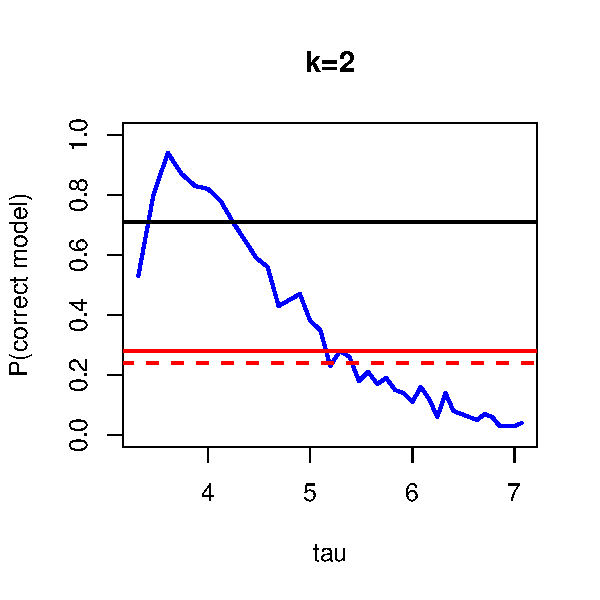
\includegraphics[width=0.32\textwidth]{Chapter-evalue/simplotmoon2}
	& 
		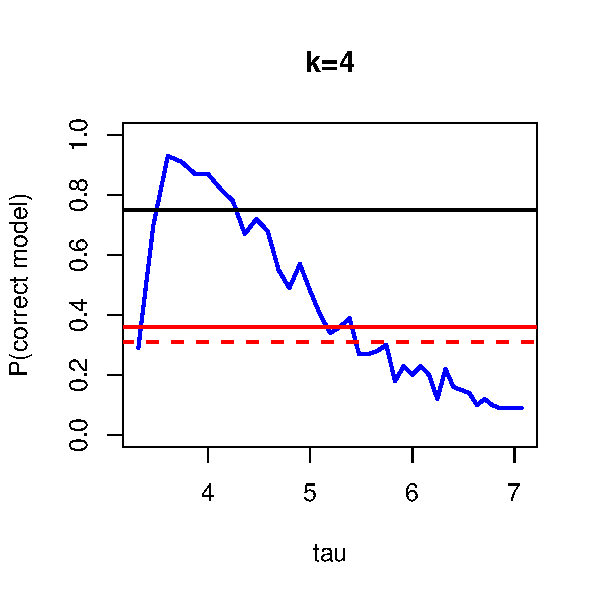
\includegraphics[width=0.32\textwidth]{Chapter-evalue/simplotmoon4} \\
	(a) & (b) \\	
		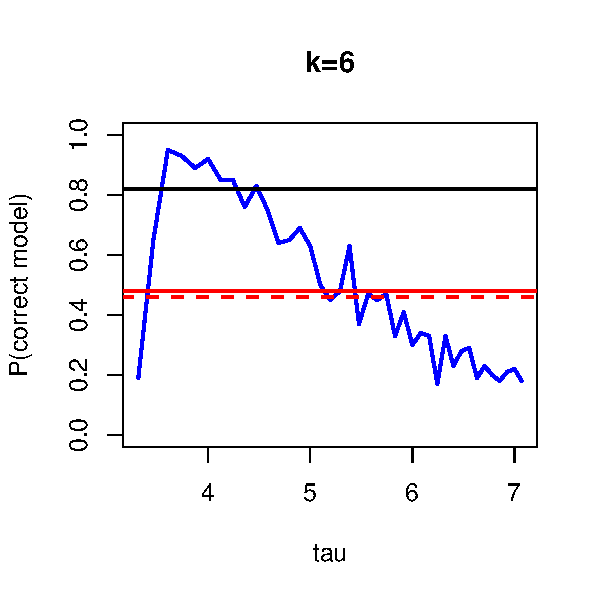
\includegraphics[width=0.32\textwidth]{Chapter-evalue/simplotmoon6}
	& 
		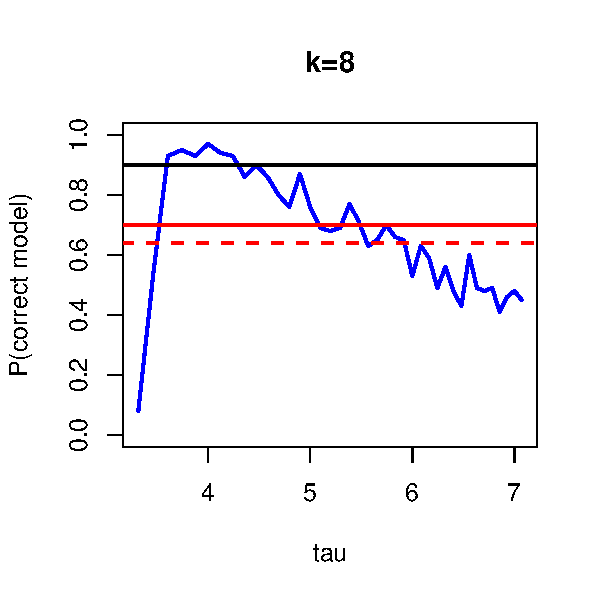
\includegraphics[width=0.32\textwidth]{Chapter-evalue/simplotmoon8} \\
	(c) & (d) \\	
\end{tabular}

\caption{Empirical probabilities of selecting the correct model through moon bootstrap for several levels of sparsity:  The $e$-values method- blue solid, AIC backward deletion- red dotted, AIC all subset- red solid, BIC backward deletion- black dotted, BIC all subset- black solid}
\label{fig:simplotsmoon}

\end{center}
\end{figure}

\begin{figure}
\begin{center}

\begin{tabular}{cc}
		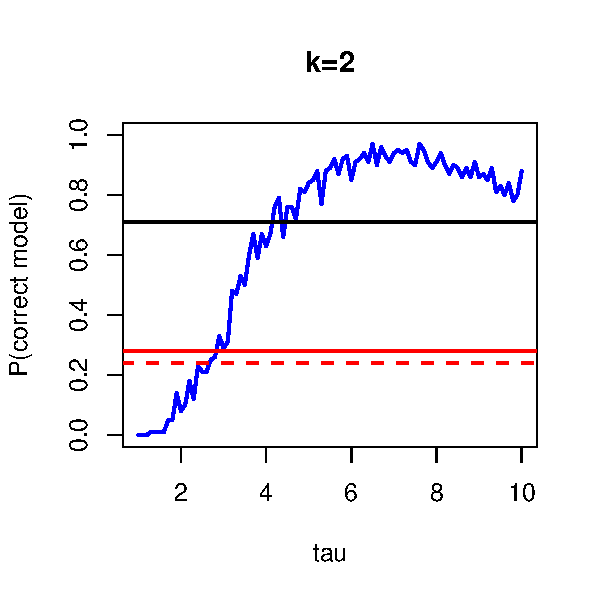
\includegraphics[width=0.32\textwidth]{Chapter-evalue/simplot_gamma2}
	& 
		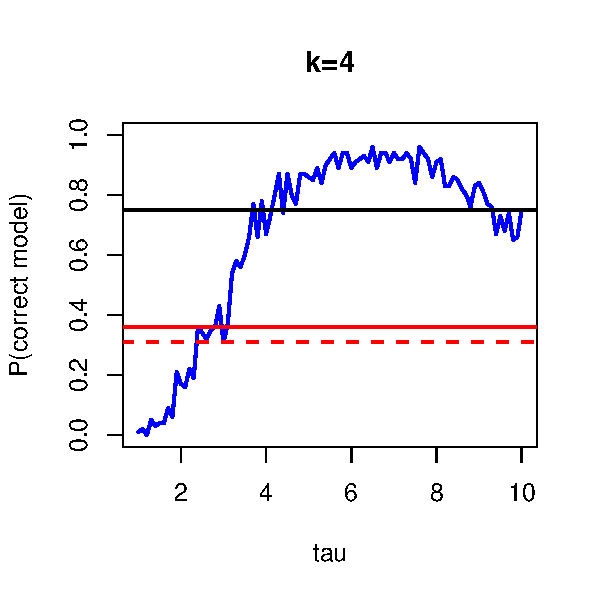
\includegraphics[width=0.32\textwidth]{Chapter-evalue/simplot_gamma4} \\
	(a) & (b) \\	
		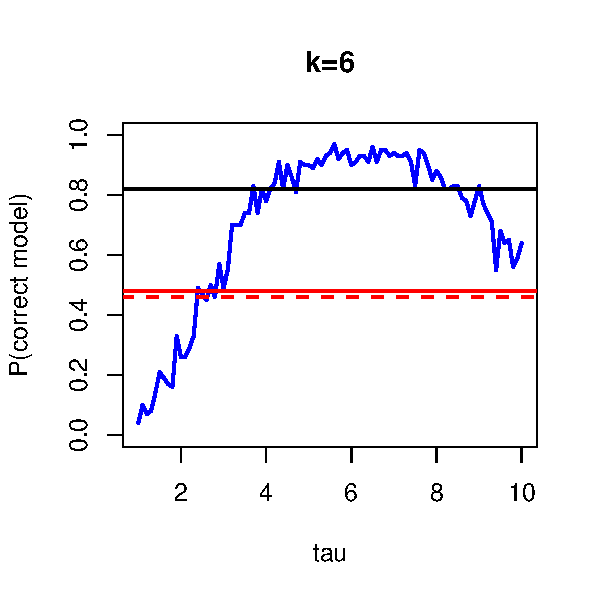
\includegraphics[width=0.32\textwidth]{Chapter-evalue/simplot_gamma6}
	& 
		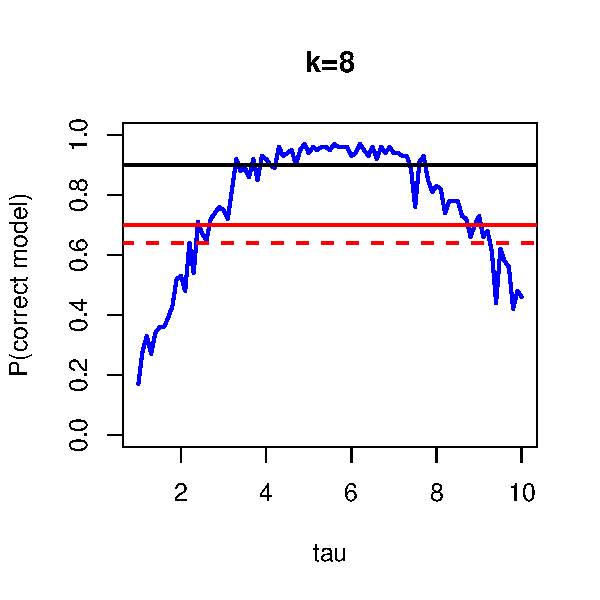
\includegraphics[width=0.32\textwidth]{Chapter-evalue/simplot_gamma8} \\
	(c) & (d) \\	
\end{tabular}

\caption{Empirical probabilities of selecting the correct model through gamma bootstrap for several levels of sparsity:  The $e$-values method- blue solid, AIC backward deletion- red dotted, AIC all subset- red solid, BIC backward deletion- black dotted, BIC all subset- black solid}
\label{fig:simplotsgamma}

\end{center}
\end{figure}

\begin{figure}
\begin{center}

\begin{tabular}{cc}
		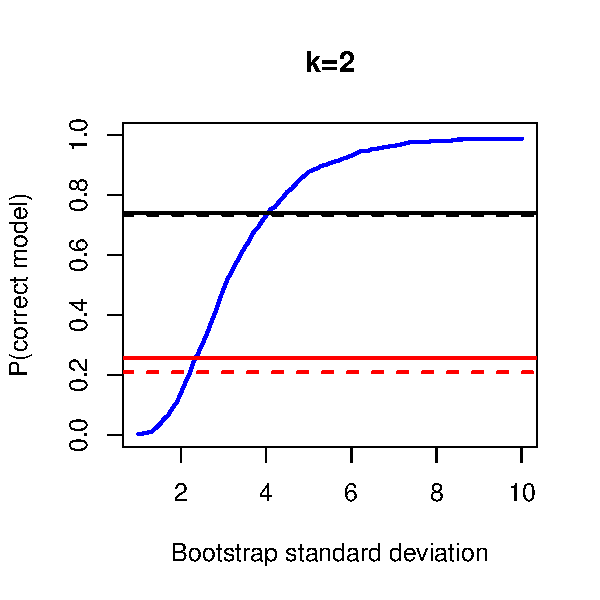
\includegraphics[width=0.32\textwidth]{Chapter-evalue/simplot2}
	& 
		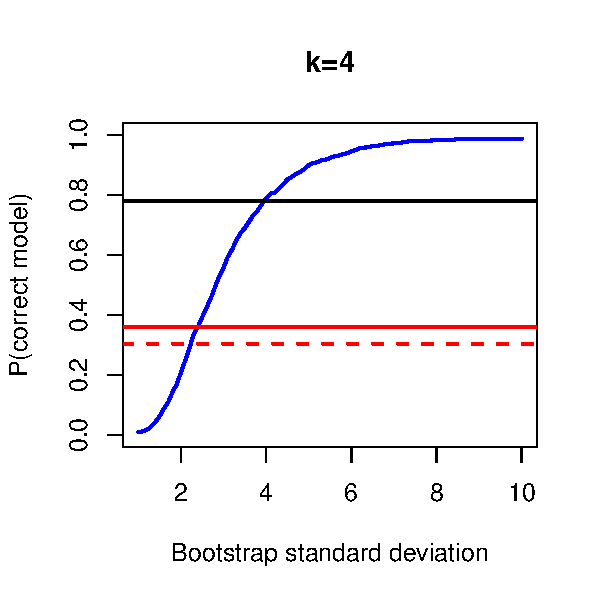
\includegraphics[width=0.32\textwidth]{Chapter-evalue/simplot4} \\
	(a) & (b) \\	
		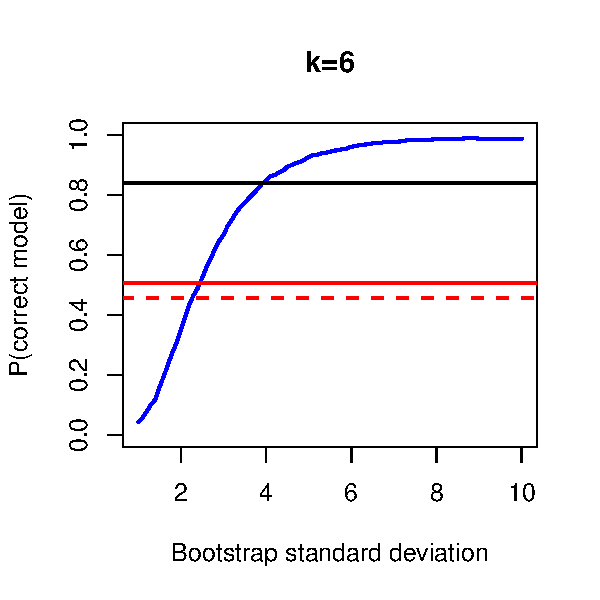
\includegraphics[width=0.32\textwidth]{Chapter-evalue/simplot6}
	& 
		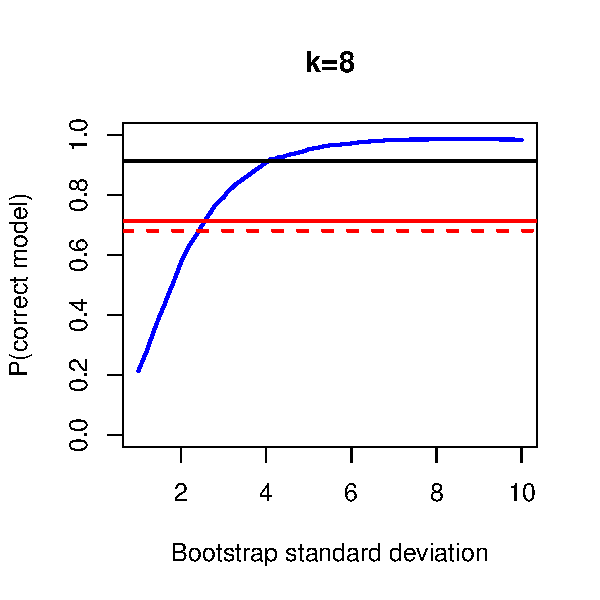
\includegraphics[width=0.32\textwidth]{Chapter-evalue/simplot8} \\
	(c) & (d) \\	
\end{tabular}

\caption{Empirical probabilities of selecting the correct model through wild bootstrap for several levels of sparsity:  The $e$-values method- blue solid, AIC backward deletion- red dotted, AIC all subset- red solid, BIC backward deletion- black dotted, BIC all subset- black solid}
\label{fig:simplotswild}

\end{center}
\end{figure}

We use the backward deletion and all-subset regression search strategies while using AIC and BIC as the model selection criterion. We use the leaps-and-bound algorithm, implemented in the {\texttt{R}} package \texttt{leaps}, for all-subset search. We display the results of this study in \ref{fig:simplotsmoon} for the moon bootstrap, in \ref{fig:simplotsgamma} for the gamma bootstrap and \ref{fig:simplotswild} for a wild bootstrap \citep{Mammen93} version of the linear regression equivalent of \ref{equation:LMMBootEqn} with i.i.d. $N(0,1)$ weights. In all three methods, and for all of $k \in \{2, 4, 6, 8 \}$ the proposed $e$-value based method performs better than AIC or BIC, as long as $\tau_{n}^{2}$ is not too small or too large. This is entirely as expected. The parametric wild bootstrap procedure has the best performance among the three, giving almost perfect detection for even very large values of $\tau_n$.
%Also interestingly, unlike the AIC or BIC, the proposed {\textit{e-value}}-based 
%procedure has the same level of accuracy in detecting the correct model regardless 
%of the amount of sparsity in $\bfbeta$. 
We experimented with other choices of $n, p, R_{1}, R_{2}$, and it seems considering $\tau \in (4, 8)$ 
in this problem ensures exact minimal adequate model selection with high chance, and typically better performance than BIC in this regard. As long as $R$ and $R_{1}$ are of the order of a few hundreds or higher, the variation from the resampling Monte Carlo step seems ignorable.

\subsection{Model selection in the presence of random effects}
Here we use the repeated measures simulation setup from \cite{PengLu12}, which has 9 fixed effects and 4 random effects, with true $\bfbeta = (0,1,1,0,0,0,0,0,0)$ and random effect covariance matrix:
%
\begin{align*}
D = \left(
	\begin{tabular}{cccc}
		9 & ~ & ~ & ~\\
		4.8 & 4 & ~ & ~\\
		0.6 & 1 & 1 & ~\\
		0 & 0 & 0 & 0\\
	\end{tabular}
	\right)
\end{align*}	
%
The error variance $\sigma^2$ is set at 1. The goal is to select the covariates of the fixed effect, thus essentially identify the covariates corresponding to the entries where $\bfbeta$ is non-zero. We use two scenarios for our study: one where the number of subjects considered is $m = 30$,  and the number of observations per subject is $n_i = 5$, and another with 60 subjects and 10 observations per subject.

%The model for the $i^\text{th}$ subject can be written as:
%%
%$$ \bfy_i = X_i \bfbeta + \bfepsilon_i $$
%%
%where $\bfepsilon_i \sim \mathcal N_{n_i} ({\bf 0}, \sigma^2 I + Z_i D Z_i^T)$. We use wild bootstrap on these residuals, so that the bootstrap equivalent of the response will be $\bfy_i^b = X_i \hat\bfbeta_{n,\text{LMM}} + u_{ib} (\bfy_i - X_i \hat\bfbeta_{n,\text{LMM}})$; with $u_{ib} \sim N(0, \tau^2)$. We take the bootstrap standard deviation $\tau = 1,2,...,8$, and determine the accuracy of our method by four measures: 

We consider $\tau \in \{1, \ldots, 15 \}$ here, and use the approximation in \ref{equation:LMMBootEqn} to calculate the bootstrapped coefficients. We consider multiple characteristics of the model that obtains the highest $e$-value, including the number of parameters it involves, the proportion of times the minimal adequate model is 
obtained, the proportion of times a zero-valued (non-zero-valued) element of beta was identified as non-zero (zero), that is, the proportion of false positives (negatives), and so on.   

In the method proposed by \cite{PengLu12}, the tuning parameter can be selected using several different criteria. We present the false positive percentage (FPR\%), false negative percentage (FNR\%) and model sizes corresponding to 
four such criteria. Our results are presented in  \ref{table:simtable1}. It can be seem the $e$-value based method handsomely outperforms the  method proposed by \cite{PengLu12}, especially in smaller sample sizes, as long as $\tau \geq 4$. 

\begin{table}[t]
	\centering
	\begin{scriptsize}
   \begin{tabular}{ll|lll|lll}
    \hline
    Method      & Tuning     & FPR\% & FNR\% & Model size & FPR\% & FNR\% & Model size \\ \cline{3-8}
    ~ & ~ & \multicolumn{3}{l|}{$n_i=5,m=30$} & \multicolumn{3}{l}{$n_i=10,m=60$}\\ \hline
  $e$-value based       & $\tau=1$      & 59.9     & 0.0   & 5.61       & 44.3     & 0.0   & 4.43       \\
    ~      & $\tau=2$      & 33.0     & 0.0   & 3.45       & 15.5     & 0.0   & 2.54       \\
    ~      & $\tau=3$      & 15.9     & 0.0   & 2.59       & 5.2      & 0.0   & 2.17       \\
    ~      & $\tau=4$      & 8.0      & 0.0   & 2.28       & 2.8      & 0.0   & 2.09       \\
    ~      & $\tau=5$      & 5.2     & 0.0   & 2.18       & 2.0   & 0.0   & 2.06       \\
    ~      & $\tau=6$      & 2.7     & 0.0   & 2.09       & 0.7   & 0.0   & 2.02       \\
    ~      & $\tau=7$      & 2.2   & 0.0   & 2.07       & 0.3   & 0.0   & 2.01       \\
    ~      & $\tau=8$      & 1.5   & 0.0   & 2.05       & 0.3   & 0.0   & 2.01       \\
    ~      & $\tau=9$      & 1.0   & 0.0   & 2.03       & 0.3   & 0.0   & 2.01       \\
    ~      & $\tau=10$      & 0.7   & 0.0   & 2.02       & 0.3   & 0.0   & 2.01       \\
    ~      & $\tau=12$      & 0.7   & 0.0   & 2.02       & 0.0   & 0.0   & 2.00       \\
    ~      & $\tau=15$      & 0.7   & 0.0   & 2.02       & 0.0   & 0.0   & 2.00       \\
     \hline
    \cite{PengLu12} & BIC    & 21.5  & 9.9   & 2.26       & 1.5   & 1.9   & 2.10       \\
    ~      & AIC    & 17    & 11.0  & 2.43       & 1.5   & 3.3   & 2.20       \\
    ~      & GCV    & 20.5  & 6     & 2.30       & 1.5   & 3     & 2.18       \\
    ~      & $\sqrt{\log n/n}$ & 21    & 15.6  & 2.67       & 1.5   & 4.1   & 2.26       \\ \hline
    \end{tabular}
    \caption{Comparison between our method and that proposed by \cite{PengLu12} through average false positive percentage, false negative percentage and model size}
    \label{table:simtable1}
    \end{scriptsize}
\end{table}
%
\begin{table}[t]
	\centering
	\begin{scriptsize}
    \begin{tabular}{llll}
    \hline
    Method          & ~ & Setting 1 & Setting 2 \\ \hline
    $e$-value based     & $\tau=1$ & 3         & 14       \\
    ~               & $\tau=2$ & 30      & 60        \\
    ~               & $\tau=3$ & 61        & 86      \\
    ~               & $\tau=4$ & 79        & 92      \\
    ~               & $\tau=5$ & 87        & 94       \\
    ~               & $\tau=6$ & 93      & 98       \\
    ~               & $\tau=7$ & 94       & 99       \\
    ~               & $\tau=8$ & 96       & 99       \\
    ~               & $\tau=9$ & 97       & 99       \\
    ~               & $\tau=10$ & 98       & 99       \\
    ~               & $\tau=12$ & 98       & 100       \\
    ~               & $\tau=15$ & 98       & 100       \\\hline
    \cite{BondellKrishnaGhosh10} & ~ & 73        & 83        \\
    \cite{PengLu12}         & ~ & 49        & 86        \\
    \cite{FanLi12}           & ~ & 90        & 100       \\ \hline
    \end{tabular}
    \caption{Comparison of our method and three sparsity-based methods of mixed effect model selection through accuracy of selecting correct fixed effects}
	\label{table:simtable2MS}
    \end{scriptsize}
\end{table}

We also compare the percentages of times the correct model was identified, and these results are presented in \ref{table:simtable2MS}, along with the corresponding results from two other papers. The proposed $e$-value based procedure performs best here for $\tau \geq 6$ for the smaller sample setting, and for $\tau\geq 12$ for larger sample setting. 



\section{Real data example}
\label{sec:regression-sec6}

\begin{figure}
%\captionsetup{justification=centering, font=footnotesize}
\begin{center}
\includegraphics[width=.8\textwidth]{Chapter-regression/cropped_gene_heatmap1}

\caption{Estimated effects of different pathway genes on the activity of genes in Mevalonate and Non-mevalonate pathways (left and right of vertical line) in \textit{A. thaliana}}
\label{fig:coeffplots}
\end{center}
\end{figure}

\begin{table}[h]
\centering
\begin{footnotesize}
\begin{tabular}{rll}
  \hline
Coeff & Gene & Pathway \\ 
  \hline
0.18 & DPPS2 & Phytosterol biosynthesis \\ 
0.14 & DPPS2 & Carotenoid biosynthesis \\ 
0.14 & DPPS2 & Flavonoid metabolism \\ 
0.11 & DPPS2 & Calvin cycle \\ 
0.11 & PPDS2mt & Phytosterol biosynthesis \\ 
0.10 & GGPPS3 & Cytokinin biosynthesis \\ 
0.10 & PPDS1 & Phytosterol biosynthesis \\ 
0.09 & DPPS3 & Flavonoid metabolism \\ 
0.09 & DPPS3 & Ubiquinone biosynthesis \\ 
0.09 & GGPPS9 & Ubiquinone biosynthesis \\ 
\hline
\end{tabular}
\caption{Top 10 gene-pathway connections in {\it A. thaliana} data found by LARN}
\label{table:coefftable}
\end{footnotesize}
\end{table}

We apply the LARN algorithm on a microarray dataset containing expression of several genes in the flowering plant \textit{Arabidopsis thaliana} \citep{WilleEtal04}. In this dataset, gene expressions are collected from $n=118$ samples, which are plants grown under different experimental conditions. We take the expressions of $q=40$ genes in two pathways for biosynthesis of isoprenoid compounds, which are key compounds affecting plant metabolism as our multiple responses. Expressions of 795 other genes corresponding to 56 other pathways are taken as predictors.

Our objective here is to find out the extent of crosstalk between isoprenoid pathway genes and those in the other pathways. We apply LARN, as well as the two methods mentioned before, on the data and evaluate them based on predictive accuracy of 100 random splits with 90 training samples. All three methods have similar mean squared prediction error (MSPE) (LARN and GL-t have MSPE 0.45 and SGL has 0.44), but LARN produces more sparse solutions on average: the mean proportion of non-zero elements in the coefficient matrix are 0.15, 0.21 and 0.29 for LARN, GL-t and SGL, respectively. Focusing on the coefficient matrix estimated by LARN, we summarize the 10 largest coefficients (in absolute values) in \ref{table:coefftable}. We also visualize coefficients corresponding to genes in the 6 pathways in the table through a heatmap in  \ref{fig:coeffplots}.

All of the four largest coefficients correspond to interactions of one gene, DPPS2, with four different pathways. Two of these pathways, Carotenoid and Phytosterol, directly use products from the isoprenoid pathways, and their connections with DPPS2 had been detected in \cite{WilleEtal04}. The large Calvin Cycle-DPPS2 coefficient reveals that compounds synthesized in Carotenoid and Phytosterol pathways get used in Calvin Cycle. 
In the heatmap, Carotenoid biosynthesis seems to be connected mostly to the non-mevalonate pathway genes (right of the vertical line), while the activities of genes in Cytokinin and Ubiquinone synthesis pathways seem to be connected with those in the mevalonate pathway. These are consistent with the findings of \cite{WilleEtal04}, \cite{FrebortEtal11} and \cite{Disch98}, respectively.

\section{Conclusion}

In this chapter we propose a class of nonconvex penalty functions, based on the idea of inverting data depths, for performing support union recovery in multitask linear regression. Although several nonconvex penalties exist in the literature, the strength of our penalization scheme lies in the significant scope of inference procedures that can rise from the choice of the reference distribution $F$. Here we consider a simplified reference distribution and provide asymptotic oracle results that ensure recovery of the non-zero row support in the coefficient matrix. We also show that a simple post-estimation thresholding recovers non-zero elements within non-zero rows of the estimated coefficient matrix with good accuracy. Although our method shares the weakness of all nonconvex penalties: small signals may go undetected or can be estimated in a biased fashion, the flexibility in choosing $F$ provides enough motivation to fine tune similar penalization schemes. Our immediate plans for future studies include extending this specific setup to generalized linear models, dimensional asymptotics assuming the data dimension $p$ to be a function of sample size $n$, as well as exploring the use of more efficient algorithms for calculating the sparse solutions, e.g. proximal gradient descent or Concave-Convex algorithms \citep{WangKimLi13}.


\newpage
\section{Proofs}
\label{section:regression-sec8}

\begin{proof}[Proof of theorem \ref{Thm:OracleThm}]

We shall prove a small lemma before going into the actual proof.

\begin{Lemma}\label{Lemma:OracleThmLemma}
For matrices $\bfK \in \mathbb R^{l \times k}, \bfL \in \mathbb R^{l \times m}, \bfM \in \mathbb R^{m \times k}$,
%
$$
\Tr (\bfK^T \bfL \bfM) = {\ve}^T (\bfK) (\bfI_k \otimes \bfL ) \ve (\bfM)
$$
%
\end{Lemma}

\begin{proof}[Proof of lemma \ref{Lemma:OracleThmLemma}]
From the property of Kronecker products, $(\bfI_k \otimes \bfL) \ve(\bfM) = \ve (\bfL\bfM)$. The lemma follows since $\Tr (\bfK^T \bfL \bfM) = \ve^T (\bfK) \ve(\bfL\bfM)$.
\end{proof}

Now, suppose $\bfB = \bfB_0 + \bfU/\sqrt n$, for some $\bfU \in \mathbb R^{p \times q}$, so that our objective function takes the form
%
\begin{eqnarray}\label{eqn:OracleThmEqn1}
T_n (\bfU) &=& \Tr \left[ \left( \bfY - \bfX\bfB_0 - \frac{1}{\sqrt n}\bfX\bfU \right)^T \left( \bfY - \bfX\bfB_0 - \frac{1}{\sqrt n}\bfX\bfU \right)\right] \notag\\
&& + \lambda_n \sum_{j=1}^p p'_F ( r_j^*) \left\| \bfb_{0j} + \frac{\bfu_j}{\sqrt n} \right\|_2 \notag\\
\Rightarrow T_n (\bfU) - T_n ({\bf 0}_{p \times q}) &=& \Tr \left[ \frac{1}{n} \bfU^T \bfX^T \bfX \bfU - \frac{2}{\sqrt n} \bfE^T \bfX\bfU\right] \notag\\
&& + \frac{\lambda_n}{\sqrt n} \sum_{j=1}^p p'_F ( r_j^*) \left( \| \sqrt n\bfb_{0j} + \bfu_j \|_2 - \| \sqrt n\bfb_{0j} \|_2 \right)  \notag\\
&=& \Tr (\bfV_1 + \bfV_2) + V_3
\end{eqnarray}

Since $\bfX^T\bfX/n \rightarrow \bfC$ by assumption, we have $\Tr(\bfV_1) \rightarrow \ve^T (\bfU)(\bfI_q \otimes \bfC) \ve(\bfU)$ using lemma \ref{Lemma:OracleThmLemma}. Using the lemma we also get
%
$$
\Tr(\bfV_2) = \frac{2}{\sqrt n} {\ve}^T(\bfE) (\bfI_q \otimes \bfX) \ve (\bfU)
$$
%
Now $\ve(\bfE) \sim \mathcal N_{nq} ({\bf 0}_n, \bfSigma \otimes \bfI_q)$, so that $(\bfI_q \otimes \bfX^T) \ve(\bfE)/\sqrt n \leadsto \bfW \equiv \mathcal N_{pq} ({\bf 0}_{pq}, \bfSigma \otimes \bfC)$ using properties of Kronecker products and Slutsky's theorem.

Let us look at $V_3$ now. Denote by $V_{3j}$ the $j$-th summand of $V_3$. Now there are two scenarios. Firstly, when $\bfb_{0j} \neq {\bf 0}_q$, we have $p'_F ( r_j^*) \stackrel{P}{\rightarrow} p'_F ( r_{0j})$. Since $\lambda_n / \sqrt n \rightarrow 0$, this implies $V_{3j} \stackrel{P}{\rightarrow} 0$ for any fixed $\bfu_j$. Secondly, when $\bfb_{0j} = {\bf 0}_q$, we have
%
$$
V_{3j} = \lambda_n n^{(s-1)/2}. (\sqrt n r^*_j )^{-s}.\frac{ p'_F ( r_j^*) \| \bfu_j \|_2 }{ (r^*_j) ^{-s}}
$$
%
We now have $\bfb^*_j = O_p(1/\sqrt n)$, and also each term of the gradient vector is $O ((r^*_j)^{-s})$ by assumption. Thus $V_{3j} = O_P( \lambda_n n^{(s-1)/2} \| \bfu_j \|_2)$. By assumption, $\lambda_n n^{(s-1)/2} \rightarrow \infty$ as $n \rightarrow \infty$, so $V_{3j} \stackrel{P}{\rightarrow} \infty$ unless $\bfu_j = {\bf 0}_q$, in which case $V_{3j} = 0$.

Accumulating all the terms and putting them into \ref{eqn:OracleThmEqn1} we see that
%
\begin{equation}
T_n(\bfU) - T_n({\bf 0}_{p \times q}) \leadsto
\begin{cases}
\ve^T (\bfU_1) [ (\bfI_q \otimes \bfC_{11}) \ve(\bfU_1) - 2 \bfW_1 ] & \text{if } \bfU_0 = {\bf 0}_{(p-p_1)q}\\
\infty & \text{otherwise}
\end{cases}
\end{equation}
where rows of $\bfU$ are partitioned into $\bfU_1$ and $\bfU_0$ according to the zero and non-zero rows of $\bfB_0$, respectively, and the random variable $\bfW$ is partitioned into $\bfW_1$ and $\bfW_0$ according to zero and non-zero \textit{elements} of $\ve (\bfB_0)$. Applying epiconvergence results of \cite{Geyer94} and \cite{KnightFu00} we now have
%
\begin{eqnarray}
\ve(\hat\bfU_{1n}) &\leadsto & (\bfI_q \otimes \bfC_{11}^{-1}) \bfW_1\label{eqn:OracleThmProofEqn2}\\
\ve(\hat\bfU_{0n}) &\leadsto & {\bf 0}_{(p-p_1)q}\label{eqn:OracleThmProofEqn3}
\end{eqnarray}
%
where $\hat\bfU_n = (\hat\bfU_{1n}^T, \hat\bfU_{0n}^T)^T := \argmin_\bfU T_n (\bfU)$.

The second part of the theorem, i.e. asymptotic normality of $\sqrt n (\ve (\hat \bfB_{1n}) - \ve(\hat\bfB_{1n})) = \hat\bfU_{1n}$ follows directly from \ref{eqn:OracleThmProofEqn2}. It is now sufficient to show that $P( \hat\bfb_j^{(1)} \neq {\bf 0}_q | \bfb_{0j} = {\bf 0}_q) \rightarrow 0$ to prove the oracle consistency part. For this notice that KKT conditions of the optimization problem for the one-step estimate indicate
%
\begin{equation}
2 \bfx_j^T (\bfY - \bfX \hat\bfB^{(1)}) = - \lambda_n p'_F (r_j^*) \frac{\bfb_j^{(1)}}{r_j^{(1)}} \quad\Rightarrow\quad \frac{2 \bfx_j^T (\bfY - \bfX \hat\bfB^{(1)})}{\sqrt n} = - \frac{\lambda_n p'_F (r_j^*)}{\sqrt n}. \frac{\bfb_j^{(1)}}{r_j^{(1)}}
\end{equation}
%
for any $1 \leq j \leq p$ such that $\hat\bfb_j^{(1)} \neq {\bf 0}_q$. Since $p'_F(r_j^*) = D^-( (r_j^*)^{-s}) = O_P ( \| (\bfb_{0j} + 1/\sqrt n \|^{-s})$ and $\lambda_n n^{(s-1)/2} \rightarrow \infty$, the right hand side goes to $-\infty$ in probability if $\bfb_{0j} = {\bf 0}_q$. As for the left-hand side, it can be written as
%
$$ \frac{2 \bfx_j^T (\bfY - \bfX \hat\bfB^{(1)})}{\sqrt n} = \frac{2 \bfx_j^T \bfX .\sqrt n (\bfB_0 - \hat\bfB^{(1)})}{n} + \frac{2 \bfx_j^T \bfE}{\sqrt n} = \frac{2 \bfx_j^T \bfX \hat\bfU_n}{n} + \frac{2 \bfx_j^T \bfE}{\sqrt n}
$$
%
Our previous derivations show that vectorized versions of $\hat\bfU_n$ and $\bfE$ have asymptotic and exact multivariate normal distributions, respectively. Hence
%
$$
\BP \left[ \hat\bfb_j^{(1)} \neq {\bf 0}_q | \bfb_{0j} = {\bf 0}_q \right] \leq P \left[ 2 \bfx_j^T (\bfY - \bfX \hat\bfB^{(1)} ) = - \lambda_n p'_F (r_j^*) \frac{\bfb_j^{(1)}}{r_j^{(1)}} \right] \rightarrow 0
$$
\end{proof}

\begin{proof}[Proof of theorem \ref{Thm:RowSupportThm}]
See the proof of corollary 2 of \cite{ObozinskiEtal11}in Appendix A therein. Our proof follows the same steps, only replacing $\bfSigma_{SS}$ with $\bfSigma \otimes \bfC_{11}$.

\end{proof}

\begin{proof}[Proof of Lemma \ref{thm:minimaxThm}]
We broadly proceed in a similar fashion as the proof of Theorem 3 in \cite{Zou06}. As a first step, we decompose the mean squared error:
%
\begin{eqnarray*}
E[ \hat\theta(F,\lambda) - \theta]^2 &=& E[ \hat\theta(F,\lambda) - z]^2 + E(z - \theta)^2 + 2 E [\hat\theta(F,\lambda) (z-\theta)] - 2E [z(z-\theta)]\\
&=& E[ \hat\theta(F,\lambda) - z]^2 + E \left[ \frac{d\hat\theta(F,\lambda)}{dz}\right] - 1
\end{eqnarray*}
%
by applying Stein's lemma \citep{Stein81}. We now use Theorem 1 of \cite{AntoniadisFan01} to approximate $\hat\theta(F,\lambda)$ in terms of $y$ only. By part 2 of the theorem,
%
\begin{equation}
\hat\theta(F,\lambda) = \begin{cases}
0 \quad & \text{if } |z| \leq \lambda p_0(F)\\
z - \text{sign}(z). \lambda D^-_1(\hat\theta(F,\lambda), F) & \text{if }|z| > \lambda p_0(F)
\end{cases}
\end{equation}
%
Moreover, applying part 5 of the theorem,
%
\begin{equation}
\hat\theta(F,\lambda) = z - \text{sign}(z).\lambda D^-_1(z, F) + o(D^-_1(z, F))
\end{equation}
%
for $|z| > \lambda p_0(F)$. Thus we get
%
\begin{equation}
[ \hat\theta(F,\lambda) - z]^2 = \begin{cases}
z^2 & \text{if } |z| \leq \lambda p_0(F)\\
\lambda^2 D^-_1(z,F)^2 + k_1(|z|) & \text{if } |z| > \lambda p_0(F)
\end{cases}
\end{equation}
%
and
%
\begin{equation}
\frac{d\hat\theta(F,\lambda)}{dz} = \begin{cases}
0 & \text{if } |z| \leq \lambda p_0(F)\\
1 +  \lambda D^-_2(z,F) + k_1'(|z|) & \text{if } |z| > \lambda p_0(F)
\end{cases}
\end{equation}
%
where $k_1(|z|) = o(|z|)$, and $D^-_2(z,F) = d^2D^-(z,F)/dz^2$. Thus
%
\begin{eqnarray}\label{eqn:MinimaxProofEqn1}
E [ \hat\theta(F,\lambda) - \theta]^2 &=& E [z^2 \BI_{|z| \leq \lambda p_0(F)}] + E \left[ \left(\lambda^2 D^-_1(|z|, F)^2 + 2 \lambda D^-_2(|z|,F) + 2 + \right.\right. \notag\\
&& \left.\left. k_1(|z|) + k_1'(|z|) \right) \BI_{|z| > \lambda p_0(F)} \right] - 1
\end{eqnarray}
%
Now
%
\begin{eqnarray*}
k_1(|z|) &=& \lambda^2 \left[ D^-_1(z,F)^2 - D^-_1(\hat\theta(F,\lambda), F)^2 \right] \quad \leq \quad \lambda^2 c_1^2, \text{ and}\\
| k_1'(|z|) | &=& \lambda \left| D^-_2(z,F) - \frac{d D^-_1(\hat\theta(F,\lambda), F)}{dz} \right| \quad \leq \quad 2\lambda c_2
\end{eqnarray*}
%
Substituting these in \ref{eqn:MinimaxProofEqn1} above we get
%
\begin{eqnarray}\label{eqn:MinimaxProofEqn2}
E [ \hat\theta(F,\lambda) - \theta]^2 & \leq & \lambda^2 p_0(F)^2 P [|z| \leq \lambda p_0(F)] + E \left[ \left(\lambda^2 f^2(|z|) + 2 \lambda D^-_2(z, F) \right) BI_{|z| > \lambda p_0(F)} \right] \notag\\
&& + \lambda^2 c_1^2 + 2\lambda c_2 + 1 \notag\\
& \leq & 2\lambda^2 c_1^2 + 4 \lambda c_2 + 1 \notag\\
& \leq & 4\lambda^2 c_1^2 + 8 \lambda c_2 + 1
\end{eqnarray}
%

Adding and subtracting $z^2 \BI_{|z| > \lambda p_0(F)}$ to the first and second summands of \ref{eqn:MinimaxProofEqn1} above, we also have
%
\begin{eqnarray}
E [ \hat\theta(F,\lambda) - \theta]^2 &=& Ez^2 + E \left[ \left(\lambda^2 D^-_1(z,F)^2 + 2 \lambda D^-_2(z,F) + 2 - y^2 + \lambda^2 c_1^2 \right.\right. \notag\\
& & \left.\left. + 2\lambda c_2 \right) \BI_{|z| > \lambda p_0(F)} \right] - 1\notag\\
& \leq & (2 \lambda^2 c_1^2 + 4 \lambda c_2) P [ |z| > \lambda p_0(F) ] + \theta^2
\end{eqnarray}
%
Following \cite{Zou06}, $P[|z| > \lambda p_0(F)] \leq 2q (\lambda p_0(F)) + 2\theta^2$, with $q(x) = \exp[-x^2/2]/(\sqrt{2\pi} x)$. Thus
%
\begin{eqnarray}
E [ \hat\theta(F,\lambda) - \theta]^2 &\leq & 2 (2 \lambda^2 c_1^2 + 4 \lambda c_2) [q (\lambda p_0(F)) + \theta^2] + \theta^2\notag\\
& \leq & (4\lambda^2 c_1^2 + 8 \lambda c_2 + 1)[q (\lambda p_0(F)) + \theta^2] 
\end{eqnarray}
%
Combining this with \ref{eqn:MinimaxProofEqn2} we get
%
\begin{equation}
E [ \hat\theta(F,\lambda) - \theta]^2 \leq [ 4(\lambda c_1 + 1)^2 - 3][q (\lambda p_0(F)) + \min(\theta^2,1)] 
\end{equation}
%
assuming without loss of generality that $c_1 \geq c_2$. Since $R(\text{ideal}) = \min(\theta^2,1)$ and $q(x) \leq (\sqrt{2\pi} x)^{-1} < 1/x$, we have the needed.
\end{proof}


\bibliographystyle{biometrics}
\bibliography{depth-regression_101316}

\clearpage
\section*{Figure and tables}

\begin{figure*}[htb]
%\captionsetup{justification=centering, font=footnotesize}
\vspace{-2em}
\begin{center}
\subfigure[]{\epsfxsize=0.31\linewidth \epsfbox{depthplot_cropped}}
\subfigure[]{\epsfxsize=0.31\linewidth \epsfbox{penalties1}}
\subfigure[]{\epsfxsize=0.31\linewidth \epsfbox{threslarn}}
\vspace{-1em}
\caption{(a) Surface and contours of a data depth function for bivariate normal distribution; (b) Comparison of L1 and SCAD \citep{FanLi01} penalty functions with depth at a scalar point: inverting the depth function helps obtain the nonconvex shape of the penalty function in the inverse depth; (c) Univariate thresholding rule for the LARN estimate (see section \ref{sec:sec4})}
\label{fig:fig1}
\end{center}
\end{figure*}

\begin{figure*}[h]
%\captionsetup{justification=centering, font=footnotesize}
\begin{center}
%\subfigure[]{\epsfxsize=0.31\linewidth \epsfbox{../../Codes/plot1log}}
%\subfigure[]{\epsfxsize=0.31\linewidth \epsfbox{../../Codes/plot2log}}
%\subfigure[]{\epsfxsize=0.31\linewidth \epsfbox{../../Codes/plot3log}}\\
\subfigure[]{\epsfxsize=0.31\linewidth \epsfbox{plot1mspe}}
\subfigure[]{\epsfxsize=0.31\linewidth \epsfbox{plot2mspe}}
\subfigure[]{\epsfxsize=0.31\linewidth \epsfbox{plot3mspe}}

\caption{Mean absolute Estimation Errors for all three methods in different $(p,q)$ settings}
\label{fig:simplots}
\end{center}
\end{figure*}

\begin{figure*}[t]
%\captionsetup{justification=centering, font=footnotesize}
\begin{center}
\includegraphics[width=\textwidth]{cropped_gene_heatmap1}

\caption{Estimated effects of different pathway genes on the activity of genes in Mevalonate and Non-mevalonate pathways (left and right of vertical line) in \textit{A. thaliana}}
\label{fig:coeffplots}
\end{center}
\end{figure*}
%

%
\begin{table}[t]
\centering
\begin{small}
    \caption{Average true positive and true negative (TP/TN) rates for 3 methods, for $n=50$ and AR1 covariance structure}
    \vspace{.1in}
    \begin{tabular}{c|ccc}
    \hline
    $\rho$ & GL-t & SGL       & LARN      \\ \hline
    \multicolumn{4}{l}{ (a) $p=20, q=20$}\\\hline
    0.9               & 0.77/0.83          & 0.92/0.99 & 0.91/0.92 \\
    0.7               & 0.81/0.83          & 0.91/0.99 & 0.89/0.93 \\
    0.5               & 0.78/0.79          & 0.89/0.99 & 0.88/0.92 \\
    0.0               & 0.85/0.78          & 0.90/0.99 & 0.90/0.91 \\ \hline
    \multicolumn{4}{l}{ (b) $p=20, q=60$}\\\hline
    0.9               & 0.90/0.66          & 0.95/0.97 & 0.89/0.92 \\
    0.7               & 0.91/0.70          & 0.93/0.96 & 0.90/0.92 \\
    0.5               & 0.80/0.69          & 0.94/0.98 & 0.93/0.92 \\
    0.0               & 0.85/0.68          & 0.93/0.97 & 0.91/0.92 \\ \hline
    \multicolumn{4}{l}{ (c) $p=60, q=60$}\\\hline
    0.9               & 0.57/0.79          & 0.68/0.99 & 0.85/0.93 \\
    0.7               & 0.50/0.79          & 0.64/0.99 & 0.83/0.93 \\
    0.5               & 0.54/0.81          & 0.64/0.99 & 0.85/0.93 \\
    0.0               & 0.58/0.79          & 0.63/0.99 & 0.84/0.93 \\ \hline
    \end{tabular}
        \end{small}
    \label{table:simtable2}
\end{table}

\begin{table}[t]
\centering
    \caption{Total runtimes in seconds for SGL and LARN algorithms for the three simulation settings}
    \vspace{.1in}
    \begin{tabular}{c|ccc}
    \hline
    Setting & GL-t & SGL    & LARN \\ \hline
    (a)     & 332 & 490    & 209  \\
    (b)       & 676 & 52  & 328 \\
    (c)       & 4994 & 39760 & 3883 \\ \hline
    \end{tabular}
    \label{table:simtimetable}
\end{table}

% latex table generated in R 3.2.4 by xtable 1.8-2 package
% Sun Oct 02 19:29:30 2016
\begin{table}[htb]
\centering
\begin{small}
\begin{tabular}{rll}
  \hline
Coeff & Gene & Pathway \\ 
  \hline
0.18 & DPPS2 & Phytosterol biosynthesis \\ 
0.14 & DPPS2 & Carotenoid biosynthesis \\ 
0.14 & DPPS2 & Flavonoid metabolism \\ 
0.11 & DPPS2 & Calvin cycle \\ 
0.11 & PPDS2mt & Phytosterol biosynthesis \\ 
0.10 & GGPPS3 & Cytokinin biosynthesis \\ 
0.10 & PPDS1 & Phytosterol biosynthesis \\ 
0.09 & DPPS3 & Flavonoid metabolism \\ 
0.09 & DPPS3 & Ubiquinone biosynthesis \\ 
0.09 & GGPPS9 & Ubiquinone biosynthesis \\ 
\hline
\end{tabular}
\end{small}
\caption{Top 10 gene-pathway connections in {\it A. thaliana} data found by LARN}
\label{table:coefftable}
\end{table}
\vspace{5em}

\end{document}
